\documentclass[../../main.tex]{subfiles}

\begin{document}

Los casos de uso representan una lista de acciones que suelen definir las interacciones entre un rol y un sistema para lograr un objetivo. Estos diagrama sirven para validar la arquitectura del sistema y verificar el sistema en desarrollo. 

\begin{figure}[H]
\centering
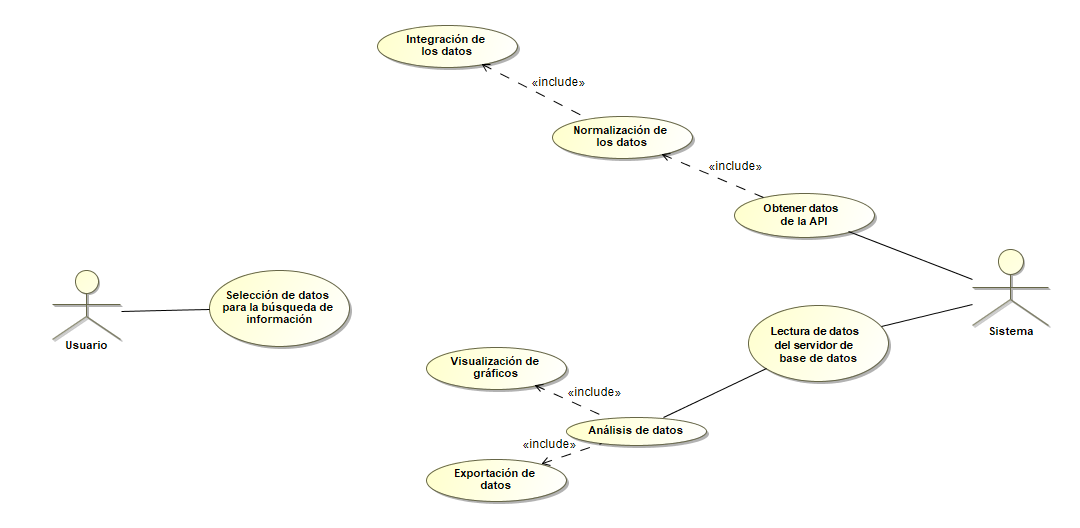
\includegraphics[width=470pt]{images/requisitos/use-case-1.png}
\caption{Casos de uso}
\end{figure}

Donde el usuario tiene la posibilidad de seleccionar los parámetros a buscar para la obtención de los datos. Del lado del sistema, este realiza la petición a la \gls{ipa} para la obtención de datos y procede a la normalización e integración de los datos. Así mismo, el sistema lee los datos presentes en el servidor de base de datos y realiza un análisis sobre el conjunto de datos obtenido.

\end{document}